\documentclass{article} % Especially this!
\usepackage[english]{babel}
\usepackage[utf8]{inputenc}
\usepackage[margin=1.5in]{geometry}
\usepackage{amsmath}
\usepackage{amsthm}
\usepackage{amsfonts}
\usepackage{amssymb}
\usepackage[usenames,dvipsnames]{xcolor}
\usepackage{graphicx}
\usepackage[siunitx]{circuitikz}
\usepackage{tikz}
\usepackage[colorinlistoftodos, color=orange!50]{todonotes}
\usepackage{hyperref}
\usepackage[numbers, square]{natbib}
\usepackage{fancybox}
\usepackage{epsfig}
\usepackage{soul}
\usepackage[framemethod=tikz]{mdframed}
\usepackage[shortlabels]{enumitem}
\usepackage[version=4]{mhchem}
\usepackage{listings}
\newcommand{\blah}{blah blah blah \dots}
\setlength{\marginparwidth}{3.4cm}


% NEW COUNTERS
\newcounter{points}
\setcounter{points}{100}
\newcounter{spelling}
\newcounter{english}
\newcounter{units}
\newcounter{other}
\newcounter{source}
\newcounter{concept}
\newcounter{missing}
\newcounter{math}
\newcounter{terms}
\newcounter{clarity}

% COMMANDS

\definecolor{myblue}{rgb}{0.668, 0.805, 0.929}
\newcommand{\hlb}[2][myblue]{ {\sethlcolor{#1} \hl{#2}} }

\newcommand{\clarity}[2]{\todo[color=CornflowerBlue!50]{CLARITY of WRITING(#1) #2}\addtocounter{points}{#1}
\addtocounter{clarity}{#1}}

\newcommand{\other}[2]{\todo{OTHER(#1) #2} \addtocounter{points}{#1} \addtocounter{other}{#1}}

\newcommand{\spelling}{\todo[color=CornflowerBlue!50]{SPELLING (-1)} \addtocounter{points}{-1}
\addtocounter{spelling}{-1}}
\newcommand{\units}{\todo{UNITS (-1)} \addtocounter{points}{-1}
\addtocounter{units}{-1}}

\newcommand{\english}{\todo[color=CornflowerBlue!50]{SYNTAX and GRAMMAR (-1)} \addtocounter{points}{-1}
\addtocounter{english}{-1}}

\newcommand{\source}{\todo{SOURCE(S) (-2)} \addtocounter{points}{-2}
\addtocounter{source}{-2}}
\newcommand{\concept}{\todo{CONCEPT (-2)} \addtocounter{points}{-2}
\addtocounter{concept}{-2}}

\newcommand{\missing}[2]{\todo{MISSING CONTENT (#1) #2} \addtocounter{points}{#1}
\addtocounter{missing}{#1}}

\newcommand{\maths}{\todo{MATH (-1)} \addtocounter{points}{-1}
\addtocounter{math}{-1}}
\newcommand{\terms}{\todo[color=CornflowerBlue!50]{SCIENCE TERMS (-1)} \addtocounter{points}{-1}
\addtocounter{terms}{-1}}


\newcommand{\summary}[1]{
\begin{mdframed}[nobreak=true]
\begin{minipage}{\textwidth}
\vspace{0.5cm}
\begin{center}
\Large{Grade Summary} \hrule 
\end{center} \vspace{0.5cm}
General Comments: #1

\vspace{0.5cm}
Possible Points \dotfill 100 \\
Points Lost (Science Terms) \dotfill \theterms \\
Points Lost (Syntax and Grammar) \dotfill \theenglish \\
Points Lost (Spelling) \dotfill \thespelling \\
Points Lost (Units) \dotfill \theunits \\
Points Lost (Math) \dotfill \themath \\
Points Lost (Sources) \dotfill \thesource \\
Points Lost (Concept) \dotfill \theconcept \\
Points Lost (Missing Content) \dotfill \themissing \\
Points Lost (Clarity of Writing) \dotfill \theclarity \\
Other \dotfill \theother \\[0.5cm]
\begin{center}
\large{\textbf{Grade:} \fbox{\thepoints}}
\end{center}
\end{minipage}
\end{mdframed}}

%#########################################################

%To use symbols for footnotes
\renewcommand*{\thefootnote}{\fnsymbol{footnote}}
%To change footnotes back to numbers uncomment the following line
%\renewcommand*{\thefootnote}{\arabic{footnote}}

% Enable this command to adjust line spacing for inline math equations.
% \everymath{\displaystyle}

\title{
\normalfont \normalsize 
\textsc{Indian Institute of Technology Bombay \\ 
CS684 Autumn Semester 2016} \\
[10pt] 
\rule{\linewidth}{0.5pt} \\[6pt] 
\huge PWM and interfacing servo motors \\
\rule{\linewidth}{2pt}  \\[10pt]
}
\author{E.R.T.S. Lab}
\date{\normalsize \today}

\begin{document}

\maketitle
\noindent

\section{Lab Objective}
\begin{enumerate}
\item 
Understand PWM operation in TMS4C123GXL.
\item
Get acquainted with interfacing servo motors with the launchpad.
\end{enumerate}

%%% Pre-requisite
\section{Pre-requisite}
\begin{enumerate}
\item Lab 1 and Lab 2: Interfacing RGB LED and both the switches.
\end{enumerate}
%%% Problem Statement
\section {Problem Statement}

% Materials go here
\textbf{Part 1:} 
In this lab you have to design RGB LED controller using SW1 and SW2 present in Launchpad
board.RGB LED controller has two modes of operation. Auto mode and Manual mode
At initial, when program is loaded controller will be in Auto mode. Combination of SW1 an SW2
has to be pressed to go to Manual mode.When Reset button is pressed, controller will go to Auto mode.

\begin{enumerate}
\item Auto mode
\begin{itemize}
  \item In Auto mode color of the RGB LED follows a pattern in a cycle.
  \item The pattern must follow the color circle as shown in Figure 1.
  \item In Auto mode SW1 will increase the speed of color transition and SW2 will decrease the speed.
\end{itemize}

\centerline{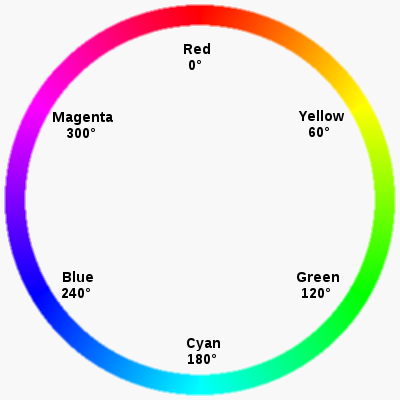
\includegraphics[scale=0.8]{RGB_color_circle.png}}
RGB Color Wheel
\footnote{Image Courtesy: https://en.wikibooks.org/wiki/File:RGB\_color\_circle.png accessed on 05/06/2016}

\item Manual mode
\begin{itemize}

\item In Manual mode, user must be able to select any one of the color from the color circle. For this
intensity of any of the 3 LEDs must be controlled independently.
\item Mode 1 (Red LED control) - When SW2 is pressed continuously(long press) and SW1 is pressed
once controller goes to Manual Mode 1. In this mode, intensity of Red LED can be controlled using
SW1 and SW2.
\item Mode 2 (Blue LED control) - When SW2 is pressed continuously(long press) and SW1 is pressed
twice controller goes to Manual Mode 2. In this mode, intensity of Blue LED can be controlled using
SW1 and SW2.
\item Mode 3 (Green LED control) - When SW1 and SW2 are pressed continuously controller goes to
Manual Mode 3. In this mode, intensity of Green LED can be controlled using SW1 and SW2.
\end{itemize}

\end{enumerate}
\textbf{Part 2:}
Interface a servo motor and control it using a switch.
\begin{enumerate}
\item When switch 1 is pressed the motor should rotate by ten degrees clockwise.
\item When switch 2 is pressed the motor should rotate by ten degrees anti-clockwise.
\item While doing the above two actions check for limits of the servo motor. It should no move beyond the operating range.
\item Also use the debouncing method that you have learned in lab 2 for interfacing the switch.
\end{enumerate}


\section {Relevant Theory}

\begin{enumerate}
\item Reference material 1 : Please go through extra resource material present in the Lab 03 folder before you proceed further.
\item Reference material 2: Please go through \href{https://www.cse.iitb.ac.in/~erts/html_pages/Resources/Tiva/TM4C123G_LaunchPad_Workshop_Workbook.pdf}{\textbf{Resources7-Chapter 15}}.
\end{enumerate}

%%%Procedure
%%%%%%%%%%%%%%%%%%%%%%%%%%%%%%
\section {Procedure}
%%%%%%%%%%%%%%%%%%%%%%%%%%%%%%
\begin{enumerate}
\item Include all the header files. Ensure that the following header file is present.\\
 include "driverlib/pwm.h"\\
 include "driverlib/timer.h"\\
 include "driverlib/interrupt.h"
 \item Configure the PORT Pins as PWM outputs and configure the PWM generator depending on the PWM pin used.
 \item  Enable the PWM output state.
 \item  Enable the PWM generator. 
\item For Part 1 - \\Depending on the color wheel switch on the respective LEDs. Do not turn off the LED completely by assigning 0 value to it as it causes it to turn ON with a high intensity. Instead assign a minimum non-zero value to it so as to reduce the intensity.   

\item For Part 2 - \\Calculate the value of PWM period. \\
eg. In this code PWM base frequency is taken as 50Hz. The total period of Servo Motor is 1/50 = 20 ms. \\ 
The oscillator frequency is 40MHz. This value is divided by 64. The answer is further divided by the PWM base frequency(50Hz).
Thus Period=12500. 

\end{enumerate}

%%% Demo and Submissions
\section {Demo and Submissions}
%%%%%%%%%%%%%%%%%%%%%%%%%%%%%%%%%%%%%%%%%%%%%%%%
Draw the state chart for the implementation of RGB LED controller.

You have to shoot two individual videos demonstrating the output the problem statement.
Your codes for each of the problem statement has to be uploaded in Github repository.


\end{document} % NOTHING AFTER THIS LINE IS PART OF THE DOCUMENT